%Stuck-at-patterns V.S. Cell-Aware Top 

%non functional requirements are those that can be used to judge the operation of a system 

%One of the first things that the graph above illustrates is that the number of non-functional test patterns decreases with as the 
%number of repetetive detects. This means that although n-detect might be helpful in order to determine the number of functional faults
%that the number of non-functional faults cannot be detected as easily by increasing the numbe of redundant fault checks. Thus, it becomes 
%aparant that the lower the number of redundant checks in the n-detect pattern set this higher the number of patterns that test the non-functional
%faults. So in order to test for non-functional faults the pattern set size, along with the test time, can be decreased by using no redundant detection.
%In other words using n0 can increase the non-functional coverage while also cutting the costs of using more redundancy with a higher n-detect pattern set. 

%%%%% All Cell-aware faults here we mentioned are not detected by stuck-at ATPG
% Page 1:
%  (1) two fault set and two differnet 10k Good-state patterns got similar results:
%  (2) # of  Non-functional patterns are more than # of functional patterns obviously, even compare with # of stuck at ATPG, it also need to add more patterns obviously, 
%  (3) but # of functional patterns V.S. # of stuck at ATPG are not very siginificantly
%  (4) Hence, we drop Non-functional patterns only add Functional patterns, we can save siginificantly costs ( time and money)
%  (5) With Multi-N-detecton functon increase,  # of  Non-functional patterns is decreasing, but not siginificantly, so,  Multi-N-detecton is helpful for saving Cell-aware fault patterns, but not too much


% Page 2:
%  (1) Equation %= # of non_functional Cell_Aware faults patterns/(stuck_at ATPG + # of funtional Cell_aware patterns)
%  (2) two fault set and two differnet 10k Good-state patterns got similar results:
% (3) With Multi-N-detecton functon increase,  % of  Non-functional cell-aware test patterns is decreasing, but when n = 3, it still remains 3%~4%, and also this decreasing is coming from the number of stuck-at ATPG increas, its real number of patterns are not dereased siginificantly (we can see in Page1)

% Page 3:
%  (1) Equation
%       (a)non_functional = # of non_functional Cell_Aware faults /(# of non_functional Cell_Aware faults+ # of functional Cell_Aware faults)
%        (b)functional = # of functional Cell_Aware faults /(# of non_functional Cell_Aware faults+ # of functional Cell_Aware faults)
%  (2) two fault set and two differnet 10k Good-state patterns got similar results:
%  (3) the non-functional Cell-Aware faults accounted for a large proportion of total of  Cell-aware faults which not detected by stuck-at ATPG
%  (4) The worst case on s12307, it accounts 100%~97%
%  (5) The best case on s38584, it still accounts 50%~55%

% From those figures(Page1~Page3), drop non-fuctional Cell-Aware faults can siginificantly enhance faults testing efficiency

%Page4, the table1
% (1) This table shows # of the funtional faults in each cicuit
% (2) The bigger circuit, the more functional faults

% Other figures in page4 and page 5
% (1) those figures are shown the number of detections for each fault mentioned in Table1
% (2) The X axis represents the each functional fault  (The order is AND=>NAND=>NOR=>OR, the input pins 2=>3=>4)
% (3) some faults are detected very lowest(1~2 times), some are largest (8000 times), those larger number of detected faults are most important for testing
% (4) Multi- N- dectection funciton cannot detected many functional faults even n increase, some of those faults are most important for testing





%%%%%%%%%%%%%%%%%%%%%%PAGE 1%%%%%%%%%%%%%%%%%%%%%%%%%%%%%%%%%%%%%%%%%%%%%%
\documentclass[12pt]{article}
\usepackage{graphicx}
\usepackage{float}
\usepackage{multirow}
\begin{document}

\begin{figure}[h!]
\begin{center}
\textbf{Stuck-At Patterns V.S. Cell-Aware Top-Off Patterns}\par\medskip
\end{center}
\begin{@twocolumntrue}
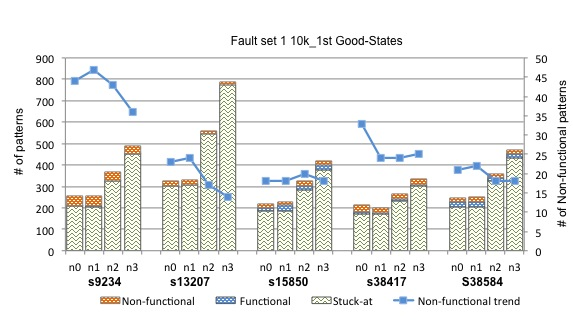
\includegraphics[scale=0.25,width=0.5\linewidth]{../top_off_set1_10k_1st.jpg}
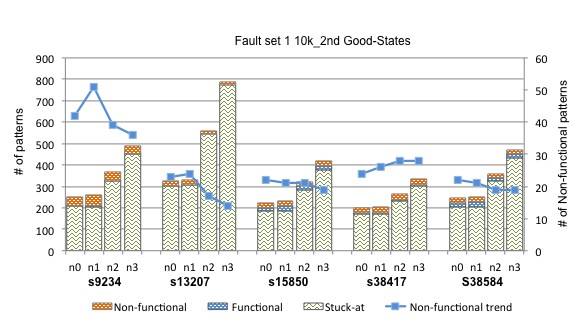
\includegraphics[scale=0.25,width=0.5\linewidth]{../top_off_set1_10k_2nd.jpg}\\ 
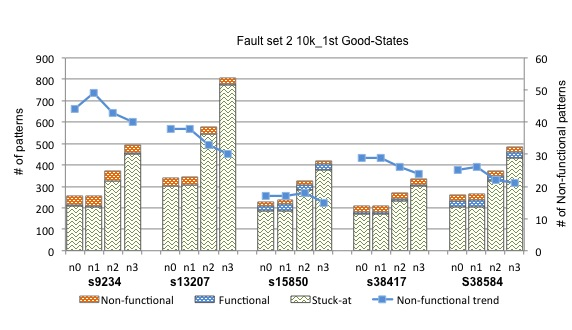
\includegraphics[scale=0.25,width=0.5\linewidth]{../top_off_set2_10k_1st.jpg}
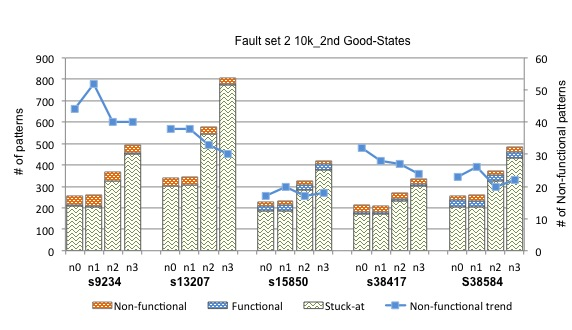
\includegraphics[scale=0.25,width=0.5\linewidth]{../top_off_set2_10k_2nd.jpg}
\end{@twocolumntrue}
\end{figure}

In the above figures we can see that two different generations of 10\,000 good-states used on two different permutations of Cell-aware fault set yielded similar results. Another observation is that in each of the four cases there are more patterns that test for non-functional defects than those that tests for functional defects that are generated by cell aware ATPG, even in comparison with the large number of patterns generated by stuck-at ATPG, the number of non-functional patterns is significant. The number of functional test patterns is negligible compared to the large amount of patterns generated by the stuck-at ATPG. Because adding all of the non-functional tests to the test set adds significant costs, these figures suggest that using n-detect with a higher degree of n can decrease the number of non-functional tests which will decrease the added costs associated with testing all of the non-functional defects. 

\begin{figure}[H]
\begin{center}
\textbf{\% Increase in Test Length When Non-Functional Cell-Aware Faults are Included in the Fault Set}\par\medskip
\end{center}
\begin{@twocolumntrue}
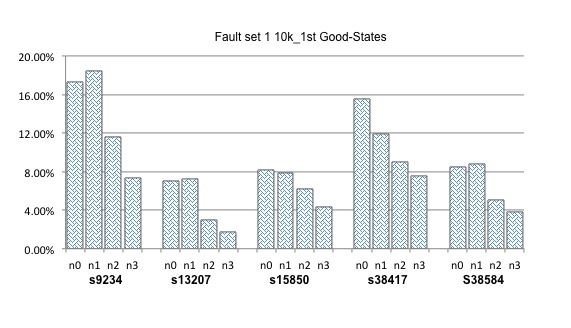
\includegraphics[scale=0.25,width=0.5\linewidth]{../percentage_increase_set1_10k_1st.jpg}
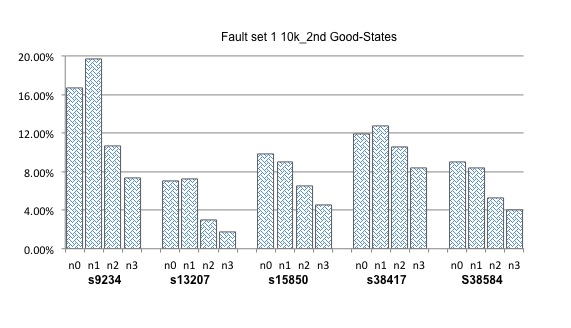
\includegraphics[scale=0.25,width=0.5\linewidth]{../percentage_increase_set1_10k_2nd.jpg}\\ 
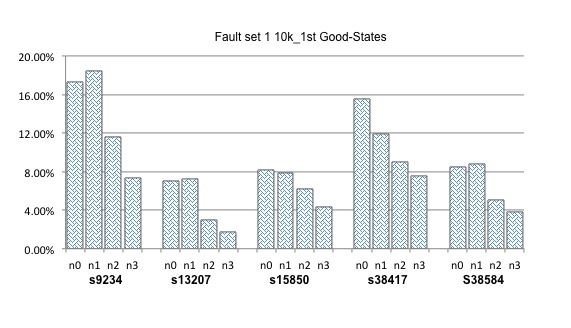
\includegraphics[scale=0.25,width=0.5\linewidth]{../percentage_increase_set1_10k_1st.jpg}
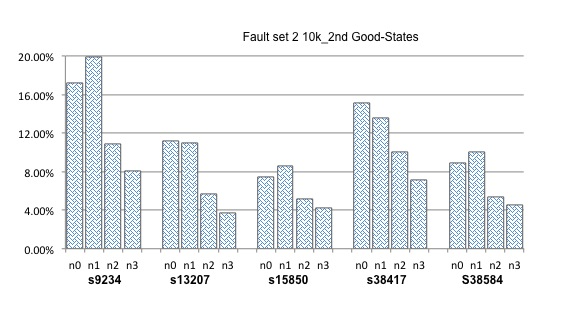
\includegraphics[scale=0.25,width=0.5\linewidth]{../percentage_increase_set2_10k_2nd.jpg}
\end{@twocolumntrue}
\end{figure}

These graphs represent the total percentage of patterns that test for non-functional defaults generated by Cell-aware ATPG out of all Stuck-at ATPG plus functional Cell-aware ATPG patterns for each of the five circuits that were tested. Here again we see that two different sets of 10\,000 good-states, as well as two different Cell-aware fault set's achieved similar results. As the n-detect redundancy increases we see a sharp decrease in the percentage of patterns that check for non-functional defects. Although even when we use n3 there remains 3~4\% of patterns testing non-functional defects this is still a dramatic decrease from the normal percentage which is around 17~18\% of all test patterns. This percentage decrease is not due to a decrease in the actual number of non-functional test patterns (as seen in figure 1), but an overall increase in the number of stuck-at ATPG patterns generated in response to the desired redundancy of the n-detect pattern generation. 

\begin{figure}[H]
\begin{center}
\textbf{Distribution of Cell-Aware Faults Between Functional & Non-Functional for those not Detected by Stuck-At ATPG}\par\medskip
\end{center}
\begin{@twocolumntrue}
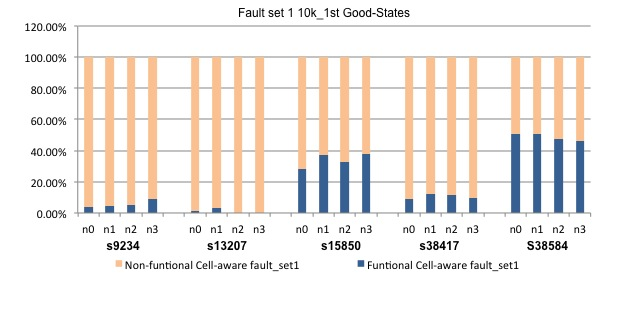
\includegraphics[scale=0.25,width=0.5\linewidth]{../distribution_set1_10k_1st.jpg}
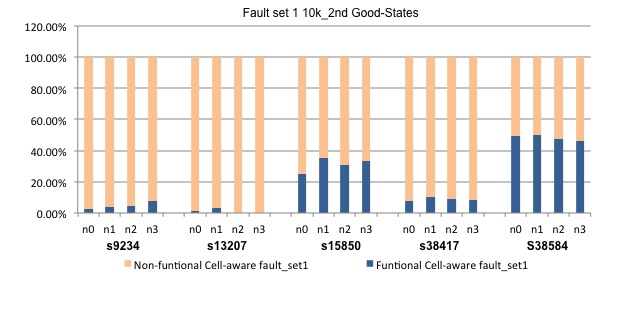
\includegraphics[scale=0.25,width=0.5\linewidth]{../distribution_set1_10k_2nd.jpg}\\ 
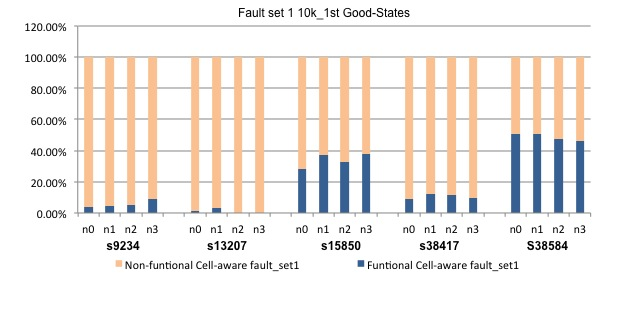
\includegraphics[scale=0.25,width=0.5\linewidth]{../distribution_set1_10k_1st.jpg}
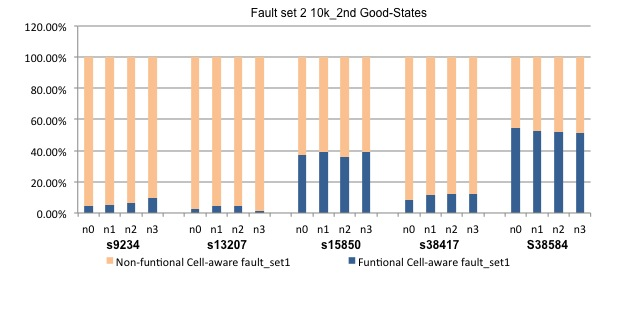
\includegraphics[scale=0.25,width=0.5\linewidth]{../distribution_set2_10k_2nd.jpg}
\end{@twocolumntrue}
\end{figure}

The above figures show the distribution of percentages of functional, and non-functional Cell-aware faults not detected by stuck-at ATPG. Once again the results were similar for all of the tested patterns and Cell-aware fault sets. Different circuits obtained different distributions based on circuits’ characters. However we can see that the non-functional Cell-aware faults that were detected accounted for a large percentage of the total Cell-aware faults for those not detected by Stack-at ATPG . In s13207 the non-functional Cell-aware faults accounted for 97-100\% of all non-detected Cell-aware faults by Stuck-at ATPG, even in s38584 non-functional Cell-aware faults accounted for 50-54\% of the total non-detected Cell-aware faults by Stuck-at ATPG. 

\begin{figure}[H]
\begin{center}
\textbf{\# of Functional Faults Table}\par\medskip
\end{center}

\noindent%\hrulefill

\smallskip\noindent
\resizebox{\linewidth}{!}{%
\begin{tabular}{|c|c|c|c|c|c|c|c|c|c|c|c|c|c|c|c|c|c|c|c|c|c|}
\hline
\multicolumn{2}{|c|}{\textbf{Benchmark}} & \multicolumn{4}{|c|}{\textbf{s9234}} & \multicolumn{4}{|c|}{\textbf{s13207}} & \multicolumn{4}{|c|}{\textbf{s15850}} & \multicolumn{4}{|c|}{\textbf{s38417}} & \multicolumn{4}{|c|}{\textbf{s38584}} \\
\hline
\multicolumn{2}{|c|}{\textbf{$n$ number}} & \textbf{n0} & \textbf{n1} & \textbf{n2} & \textbf{n3} & \textbf{n0} & \textbf{n1} & \textbf{n2} & \textbf{n3} & \textbf{n0} & \textbf{n1} & \textbf{n2} & \textbf{n3} & \textbf{n0} & \textbf{n1} & \textbf{n2} & \textbf{n3} & \textbf{n0} & \textbf{n1} & \textbf{n2} & \textbf{n3} \\
\hline
\multirow{2}{*}{Fault Set 1} & 10k 1st & 4 & 5 & 5 & 7 & 1 & 3 & 0 & 0 & 26 & 41 & 31 & 37 & 26 & 38 & 31 & 23 & 153 & 177 & 142 & 128 \\ \cline{2-22} & 10k 2nd &3 &4 &4	&6 &1 &3 &0 &0 &23 &39 &29 &33 &21 &33 &24 &20 &149 &175 &141 &128	\\ 
\hline
\multirow{2}{*}{Fault Set 2} & 10k 1st & 5&7&7&8&2&4&4&1&41&53&45&47&35&46&45&36&183&216&178&160	
 \\ \cline{2-22} & 10k 2nd & 5&6&6&8&2&5&4&1&41&47&39&44&23&36&33&30&190&212&177&163
	\\ 
\hline
\end{tabular}}
\end{figure}
This table shows the number of functional Cell-aware faults in each circuit, because Cell-aware faults are inserted in each of the gates we can see that the larger the circuit, the more functional Cell-aware faults are inserted.


\begin{figure}[H]
\begin{center}
\textbf{Number of Detections for each Fault Detected by Good-State Patterns}\par\medskip
\end{center}
\begin{@twocolumntrue}
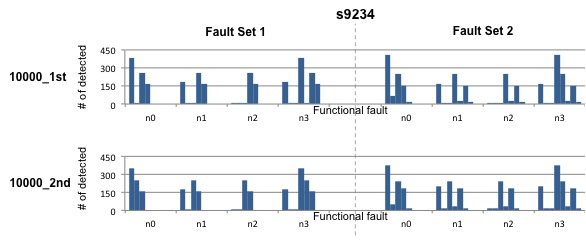
\includegraphics[scale=0.25,width=0.5\linewidth]{../detections_s9234.jpg}
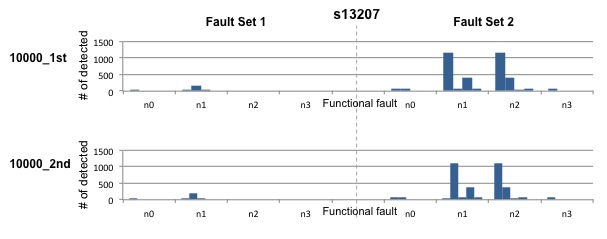
\includegraphics[scale=0.25,width=0.5\linewidth]{../detections_s13207.jpg}\\ 
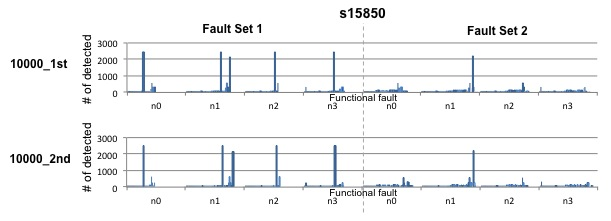
\includegraphics[scale=0.25,width=0.5\linewidth]{../detections_s15850.jpg}
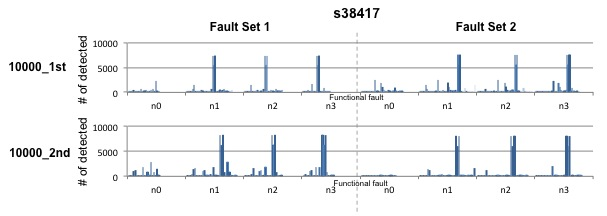
\includegraphics[scale=0.25,width=0.5\linewidth]{../detections_s38417.jpg}
\end{@twocolumntrue}
\begin{center}
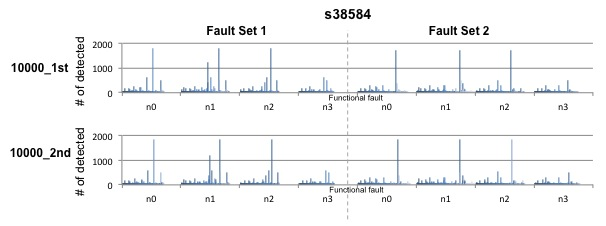
\includegraphics[scale=0.25,width=0.5\linewidth]{../detections_s38584.jpg}
\end{center}
\end{figure}


Here are charts for each of the five circuits that were tested. They show the number of functional faults that were detected based on Cell-aware fault sets used and the iteration of the test. The bars above each of the n-detect numbers represent the faults detected in each set of gates: AND, NAND, NOR, and OR respectively, with 2,3, and 4 input pins each. We noticed that some faults were detected only 2 or 3 times, whereas others were detected as many as 8\,000 times. The faults that were detected many times are likely the most crucial faults. N-detect does not detect many important functional faults, even as n increases. This suggests that increasing the redundancy of the test set with n-detect is ineffective for examining these crucial functional faults. 

\end{document}



















